\documentclass[12pt]{article}
%\usepackage[utf8]{inputenc}
%\documentclass[UTF8]{ctexart}
%\usepackage[UTF8, heading = false, scheme = plain]{ctex}
\usepackage{geometry}
%geometry{a4paper,scale=0.9}
\geometry{a4paper,left=1cm,right=1cm,top=1cm,bottom=2cm}
\usepackage{amsfonts}
\usepackage{color}
\usepackage{url}
%\usepackage{biblatex}
\usepackage{amsmath}
\usepackage{amssymb}
\usepackage{latexsym}
\usepackage{cite}
%\addbibresource{ref.bib}
%\bibliography{ref.bib}
\usepackage{caption}
\usepackage{graphicx, subfig}
\usepackage{float}
%\usepackage[fontset=ubuntu]{ctex}
%\usepackage{fontspec}
\usepackage{xeCJK}
%\usepackage[colorlinks,
%anchorcolor=black,
%citecolor=black]{hyperref}
%\setmainfont{SimSun}
\usepackage[section]{placeins}
\usepackage{enumitem}
\usepackage{framed}
\usepackage[framemethod=TikZ]{mdframed}
\usepackage{indentfirst}
\usepackage{setspace}%使用间距宏包
\linespread{1.5}
%\title{预备知识}
%\author{leolinuxer }
%\date{June 2020}

\title{信号变换相关:傅里叶变换等}
%\author{leolinuxer }
%\date{June 2020}

\begin{document}
\maketitle

\section{傅里叶级数\cite{Understand_Fourier_Series_Ma}}
\subsection{对周期函数进行分解的思路}
假设$f(x)$是周期为$T$的函数,那么要怎么构造三角函数的和,使之等于 $f(x)$?
\subsubsection{常数项}
对于$y=C,C\in\mathbb{R}$这样的常数函数,根据周期函数的定义,常数函数是周期函数,周期为任意实数。所以,\textbf{分解里面得有一个常数项。}

\subsubsection{通过$\sin(x),\cos(x)$进行分解}
选择 $\sin(x),\cos(x)$ 的原因:
\begin{itemize}
    \item 它们是周期函数,进行合理的加减组合,结果可以是周期函数;
    \item 它们的微分和积分都很简单;
    \item 它们都是“对称函数”:$\sin(x)$ 是奇函数,$\cos(x)$ 是偶函数,并且任意函数可以分解和奇偶函数之和:$f(x) = \frac{f(x)+f(-x)}{2} + \frac{f(x)-f(-x)}{2} = f_{even} + f_{odd}$ 
\end{itemize}

\subsubsection{保证组合出来周期为$T$}
之前说了,$f(x)$是周期为$T$的函数,我们怎么保证组合出来的函数周期依然为$T$呢?

比如某个函数的周期为$2\pi$。很显然,$\sin(x)$的周期也是$2\pi$,并且 $\sin(2x)$的周期也是$2\pi$,(虽然最小周期是$\pi$);很显然,$sin(nx),n\in\mathbb{N}$的周期都是$2\pi$。

更一般的,如果$f(x)$的周期为$T$,那么:$\sin(\frac{2\pi n}{T}x), \cos(\frac{2\pi n}{T}x), n\in\mathbb{N}$ 这些函数的周期都为$T$。

将这些函数进行加减,就保证了得到的函数的周期也为$T$。

\subsubsection{调整振幅}
现在我们有一堆周期为$2\pi$的函数了,比如说$sin(x),sin(2x),sin(3x),sin(4x),sin(5x)$,通过调整振幅可以让它们慢慢接近目标函数。

\subsubsection{小结}
综上,构造出来的三角函数之和大概类似下面的样子:
$$
f(x) = C + \sum_{n=1}^{+\infty}\big(a_n\cos{(\frac{2\pi n}{T}}x) + b_n\sin(\frac{2\pi n}{T}x)\big), C \in \mathbb{R}
$$

这样就符合之前的分析:
\begin{itemize}
    \item 有常数项
    \item 奇函数和偶函数可以组合出任意函数
    \item 周期为T
    \item 调整振幅,逼近原函数
\end{itemize}

接下来需要确定这三个系数:$C, {a_n}, {b_n}$

\subsection{$\sin(x)$的另外一种表示方法}
直接不好确定,要迂回一下,先稍微介绍一下什么是:$e^{i\omega  t}$

\subsubsection{$e^{i\omega t}$介绍}
看到类似于$e^{i\theta}$这种表达式,就应该想到复平面上的一个夹角为$\theta$ 的向量:
\begin{figure}[H]
  \centering
  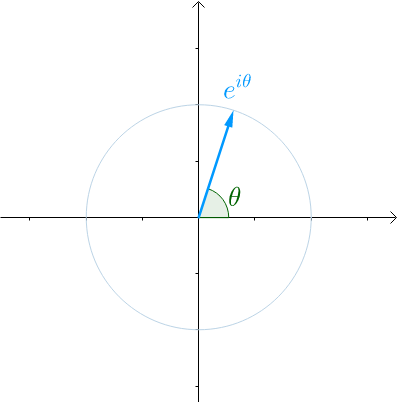
\includegraphics[width=.3\textwidth]{fig/eitheta图像.png} 
\end{figure}
那么当$\theta$不再是常数,而是代表时间的变量$t$的时候,$e^{i\theta}\to e^{i{\color{red}t}}$
随着时间$t$的流逝,从0开始增长,这个向量就会旋转起来,$2\pi$秒会旋转一圈,也就是$T=2\pi$。

\subsubsection{通过$e^{i\omega t}$表示$\sin(t)$}
根据欧拉公式,有$e^{it} = \cos(t)+i\sin(t)$

所以,在时间$t$轴上,把$e^{it}$向量的虚部(也就是纵坐标)记录下来,得到的就是$\sin(t)$;在时间$t$轴上,把$e^{i2t}$向量的虚部记录下来,得到的就是$\sin(2t)$;如果在时间$t$轴上,把$e^{it}$的实部(横坐标)记录下来,得到的就是$\cos(t)$的曲线;

更一般的我们认为,我们具有两种看待$sin(x),cos(x)$的角度:
$$
e^{i\omega t} \Longleftrightarrow \begin{cases}
\sin(\omega t)\\
\cos(\omega t)
\end{cases}
$$

这两种角度,一个可以观察到旋转的频率,所以称为频域;一个可以看到流逝的时间,所以称为时域:
\begin{figure}[H]
  \centering
  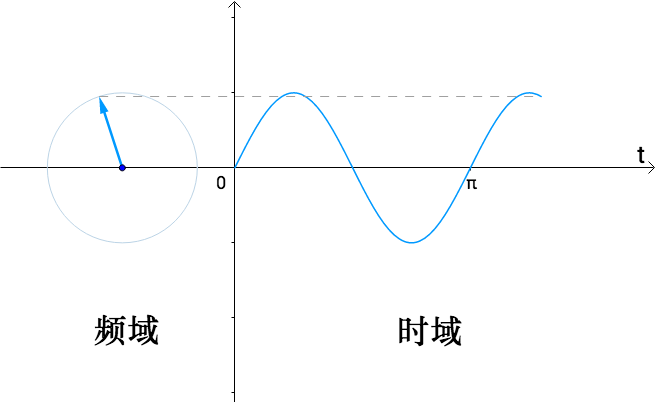
\includegraphics[width=.5\textwidth]{fig/频域和时域对比图.png} 
\end{figure}

\subsection{通过频域来求系数}
\subsubsection{函数是线性组合}
假设有这么个函数:$g(x)=\sin(x)+\sin(2x)$是一个$T=2\pi$的函数,如果转到频域去,那么它们是下面这个复数函数的虚部:$e^{it}+e^{i2t}$。

先看看$e^{i\theta}+e^{i2\theta}$,其中$\theta$是常数,很显然这是两个向量之和:
\begin{figure}[H]
  \centering
  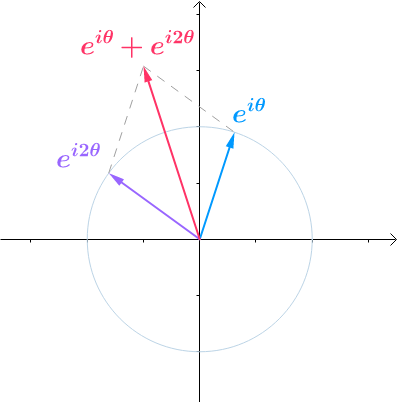
\includegraphics[width=.5\textwidth]{fig/eitheta向量和.png} 
\end{figure}

现在让它们动起来,把$\theta$变成流逝的时间$t$,并且把虚部记录下来:
\begin{figure}[H]
  \centering
  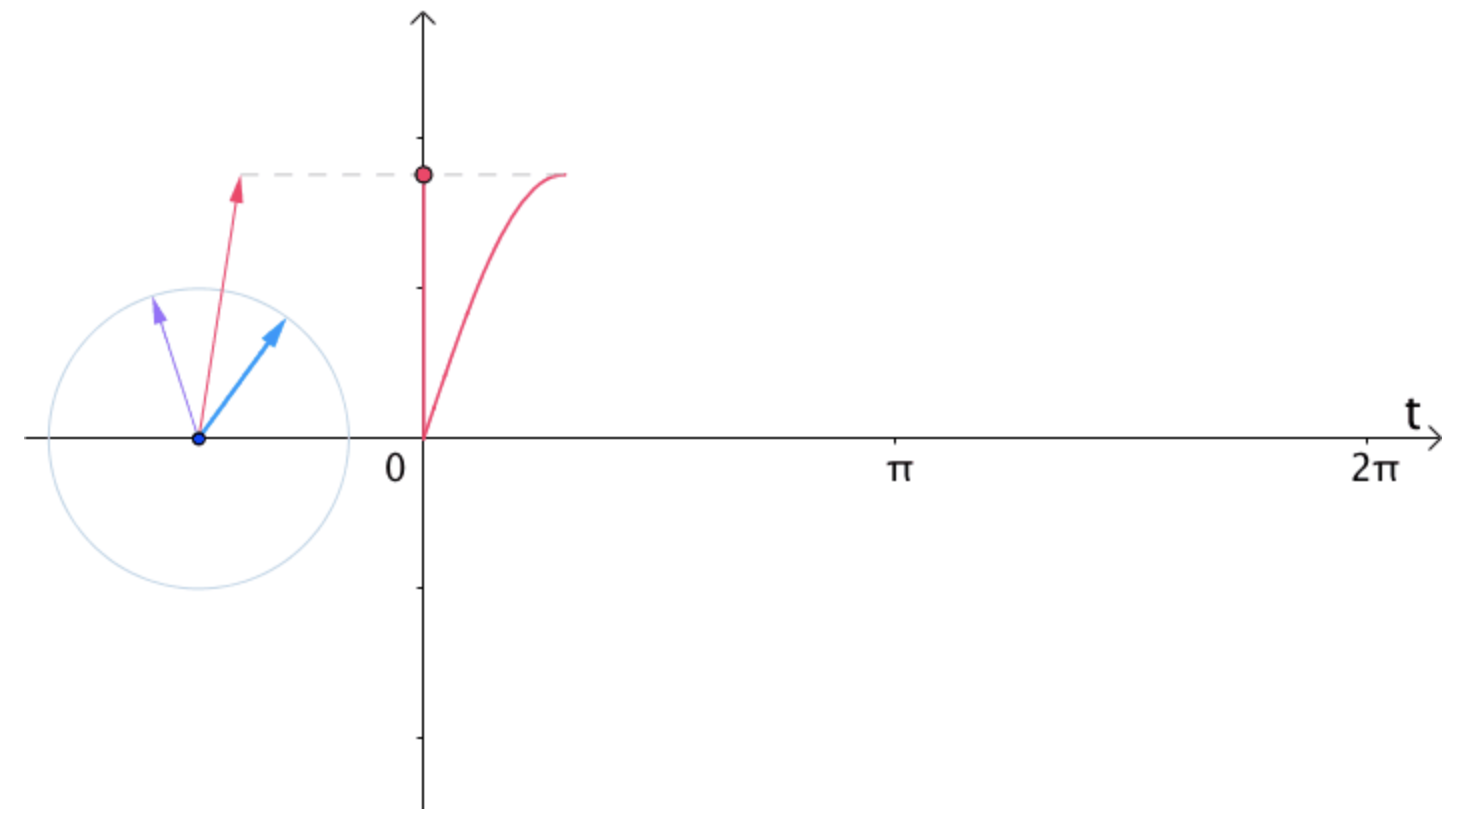
\includegraphics[width=.5\textwidth]{fig/eitheta向量和动态1.png} 
\end{figure}
\begin{figure}[H]
  \centering
  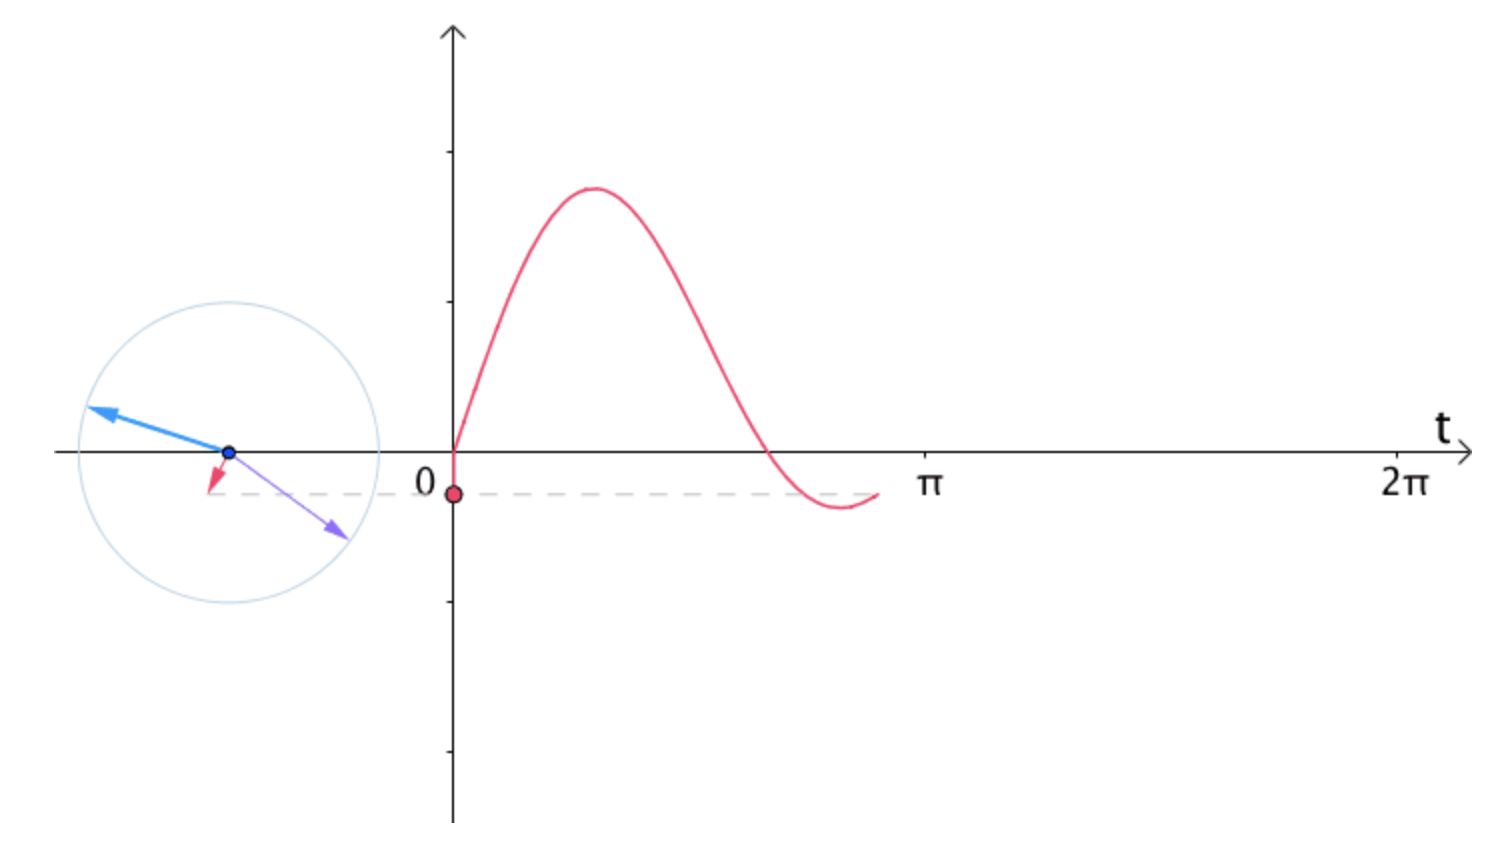
\includegraphics[width=.5\textwidth]{fig/eitheta向量和动态2.png} 
\end{figure}
\begin{figure}[H]
  \centering
  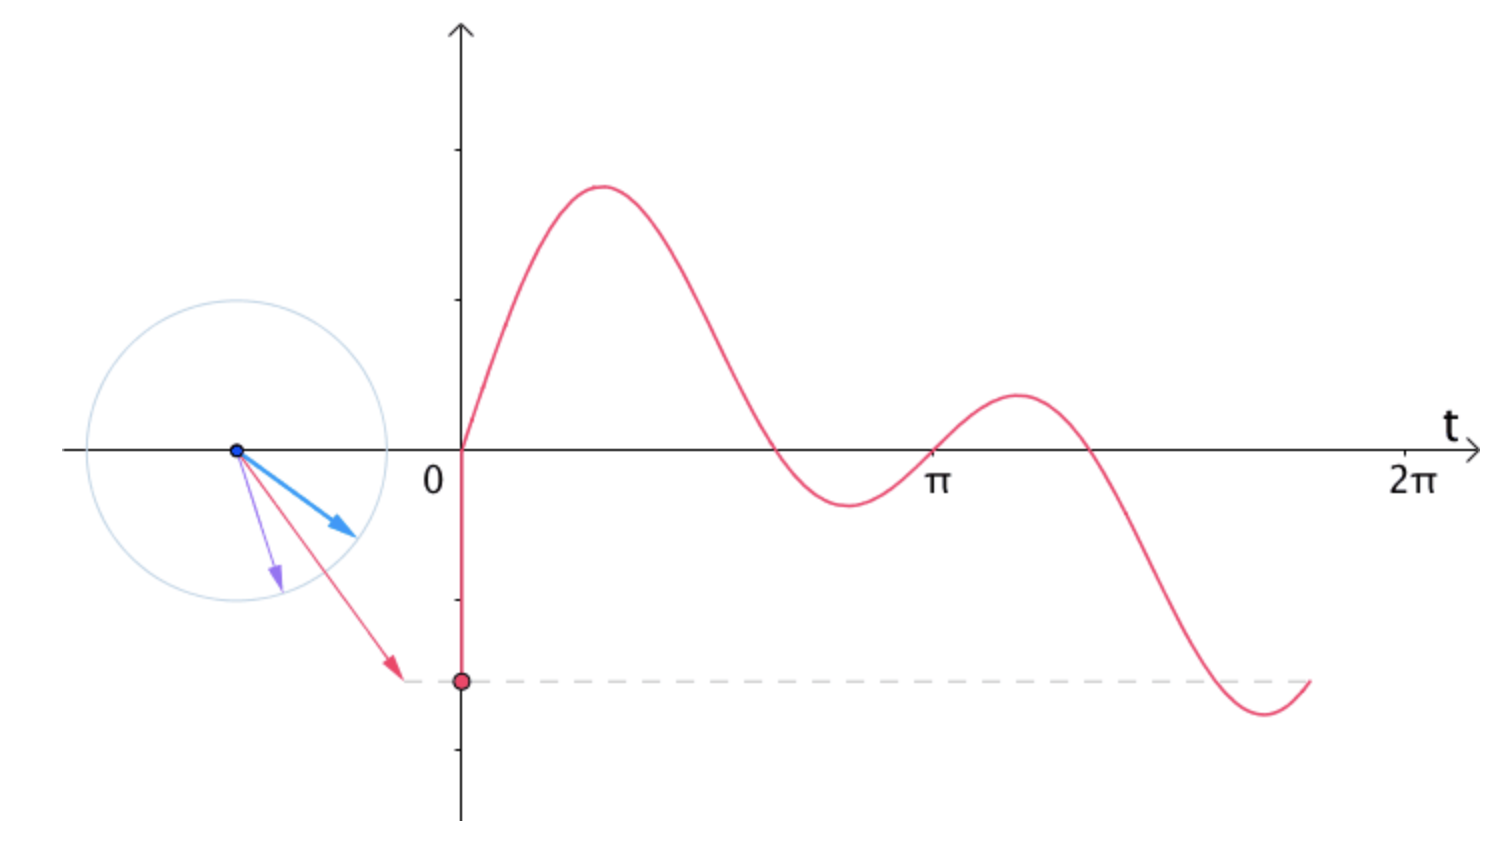
\includegraphics[width=.5\textwidth]{fig/eitheta向量和动态3.png} 
\end{figure}

我们令:$G(t)=e^{it}+e^{i2t}$这里用大写的G来表示复数函数。刚才看到了,$e^{it}$和$e^{i2t}$都是向量,所以上式可以写作:
$$
\overrightarrow{G(t)}=\overrightarrow{e^{it}}+\overrightarrow{e^{i2t}}
$$

这里就是理解的重点了,从线性代数的角度:
$e^{it}$和$e^{i2t}$是基,$G(t)$是基$e^{it},e^{i2t}$的线性组合。

定义$g(t)$是$G(t)$的虚部,所以取虚部,很容易得到:
$$\overrightarrow{g(t)}=\overrightarrow{sin(t)}+\overrightarrow{sin(2t)}$$
即$g(t)$是基$\sin(t),\sin(2t)$的线性组合。

那么$\sin(t),\sin(2t)$的系数,实际上是$g(t)$在基$\sin(t),\sin(2t)$下的坐标了。

\subsubsection{如何求正交基的坐标}
有了这个结论之后,我们如何求坐标?
我们来看个例子,假设:
$\vec{w_{}}=2\vec{u_{}}+3\vec{v_{}}$
其中$\vec{u_{}}=\begin{pmatrix}1\\1\end{pmatrix},\vec{v_{}}=\begin{pmatrix}-1\\1\end{pmatrix}$
通过点积(关于点积可以参考如何理解协方差、相关系数和点积?):
因为$\vec{u_{}}\cdot \vec{v_{}}=0$
可知这两个向量正交,是正交基。

通过点积可以算出$\vec{u_{}}$的系数(对于正交基才可以这么做):
$$
\frac{\vec{w_{}}\cdot \vec{u_{}}}{\vec{u_{}}\cdot \vec{u_{}}}=\frac{(1,5)\cdot(-1,1)}{(-1,1)\cdot(-1,1)}=2
$$

\subsubsection{如何求sin(nt)基下的坐标}
在这里抛出一个结论(可以参考\url{https://ccjou.wordpress.com/2009/08/18/%E5%BE%9E%E5%B9%BE%E4%BD%95%E5%90%91%E9%87%8F%E7%A9%BA%E9%96%93%E5%88%B0%E5%87%BD%E6%95%B8%E7%A9%BA%E9%96%93/}[從幾何向量空間到函數空間]),函数向量的点积是这么定义的:
$$
\overrightarrow{f(x)}\cdot\overrightarrow{g(x)}=\int_{0}^{T}f(x)g(x)dx
$$

其中,$f(x)$是函数向量,$g(x)$是基,$T$是$f(x)$的周期。

那么对于:
$$
g(x)=sin(x)+sin(2x)
$$
其中,$g(x)$是向量,$\sin(t),\sin(2t)$是基,周期$T=2\pi$。

因为根据刚才内积的定义:
$$
\overrightarrow{\sin(t)}\cdot\overrightarrow{\sin(2t)}=\int_{0}^{2\pi}\sin(t)\sin(2t)dt=0
$$
所以$\sin(t),\sin(2t)$是正交基。

那么根据刚才的分析,可以这么求坐标:
$$
\frac{\overrightarrow{g_{}}\cdot \overrightarrow{sin(t)}}{\overrightarrow{sin(t)}\cdot \overrightarrow{sin(t)}}=\frac{\int_{0}^{2\pi}g(x)sin(x)dx}{\int_{0}^{2\pi}sin^2(x)dx}=1
$$

\subsubsection{更一般的情况}
对于我们之前的假设,其中$f(x)$周期为$T$:
$$
f(x)=C+\sum _{{n=1}}^{\infty}\left(a_{n}cos({\frac{2\pi n}{T}x})+b_{n}sin({\frac{2\pi n}{T}x})\right),C\in\mathbb{R}
$$

可以改写为:
$$
f(x)=C\cdot 1+\sum _{{n=1}}^{\infty}\left(a_{n}cos({\frac{2\pi n}{T}x})+b_{n}sin({\frac{2\pi n}{T}x})\right),C\in\mathbb{R}
$$

也就是说向量$f(x)$的基为:
$$
\{1,cos({\frac{2\pi n}{T}x}),sin({\frac{2\pi n}{T}x})\}
$$
是的,1也是基。那么可以得到:
$$
a_n=\frac{\int_{0}^{T}f(x)cos({\frac{2\pi n}{T}x})dx}{\int_{0}^{T}cos^2({\frac{2\pi n}{T}x})dx}=\frac{2}{T}\int_{0}^{T}f(x)cos({\frac{2\pi n}{T}x})dx
$$
$$
b_n=\frac{\int_{0}^{T}f(x)sin({\frac{2\pi n}{T}x})dx}{\int_{0}^{T}sin^2({\frac{2\pi n}{T}x})dx}=\frac{2}{T}\int_{0}^{T}f(x)sin({\frac{2\pi n}{T}x})dx
$$

$C$也可以通过点积来表示,最终我们得到:
$$
f(x)={\frac{a_{0}}{2}}+\sum _{{n=1}}^{\infty}\left(a_{n}\cos({\tfrac  {2\pi nx}{T}})+b_{n}\sin({\tfrac  {2\pi nx}{T}})\right)
$$
其中:
$$
a_{n}={\frac  {2}{T}}\int _{{x_{0}}}^{{x_{0}+T}}f(x)\cdot \cos({\tfrac  {2\pi nx}{T}})\ dx, n\in\{0\}\bigcup\mathbb{N}
$$
$$
b_{n}={\frac  {2}{T}}\int _{{x_{0}}}^{{x_{0}+T}}f(x)\cdot \sin({\tfrac  {2\pi nx}{T}})\ dx, n\in\mathbb{N}
$$

\section{傅里叶变换\cite{Understand_Fourier_Transform_Ma}}
\subsection{通俗地理解傅立叶变换}
1666年牛顿发现太阳光经三棱镜的折射后可呈现彩色光,称为光的色散现象。而光是一种波,而光的颜色由振幅和频率所决定。所以色散实际上是,白色的光波被分解为七色光波(实际应该是无数种颜色的光波):

七色光波可以用正弦波$a_n\sin(nx)$(其中$a_n$是振幅,$nx$可以表示频率)来近似。因此光被分解后的颜色实际就对应了傅立叶级数(下面只是傅立叶级数的非常不准确的近似,为了帮助理解简化成了这样子,让我心中充满了罪恶感,后面会给出严格定义):
$$
\text{白色} = \sum\underbrace{{a_n}\sin(nx)}_{\text{各色颜色对应的傅里叶级数}}
$$

\subsection{时域:旋转与傅立叶级数}
根据[傅里叶级数]一节的推导,给定周期为$T$的函数$f(x)$,并且$f(x)$满足傅立叶级数的收敛条件,那么可以写作傅立叶级数:
$$
f(x)={\frac{a_{0}}{2}}+\sum _{{n=1}}^{\infty}\left(a_{n}\cos({\tfrac  {2\pi nx}{T}})+b_{n}\sin({\tfrac  {2\pi nx}{T}})\right)
$$

其中:
$$
a_{n}={\frac  {2}{T}}\int _{{x_{0}}}^{{x_{0}+T}}f(x)\cdot \cos({\tfrac  {2\pi nx}{T}})\ dx
$$
$$
b_{n}={\frac  {2}{T}}\int _{{x_{0}}}^{{x_{0}+T}}f(x)\cdot \sin({\tfrac  {2\pi nx}{T}})\ dx
$$

\subsubsection{欧拉公式}
根据欧拉公式:
$$
e^{i\theta } = \cos \theta +i\sin \theta 
$$

我们可以推出:
$$
    \sin \theta ={\frac{e^{{i\theta }}-e^{{-i\theta }}}{2i}} 
$$
$$
    \cos \theta ={\frac{e^{{i\theta }}+e^{{-i\theta }}}{2}}
$$

根据上式,我们可以写出傅立叶级数的另外一种形式:
$$
f(x)=\sum _{{n=-\infty}}^{\infty}c_{n}\cdot e^{{i{\tfrac  {2\pi nx}{T}}}}
$$

其中:
$$
c_{n}={\frac{1}{T}}\int _{{x_{0}}}^{{x_{0}+T}}f(x)\cdot e^{{-i{\tfrac  {2\pi nx}{T}}}}\ dx
$$

同样的,看到类似于$e^{i\theta}$这种就应该想到旋转,从这角度来看,傅立叶级数:
$$
f(x)=\sum _{{n=-N}}^{N}c_{n}\cdot e^{{i{\tfrac  {2\pi nx}{T}}}}
$$
实际上就是说,曲线可以理解为无数旋转的叠加,这怎么理解呢?

\subsubsection{火星的轨迹曲线}
比如这是地球上观察到的火星运行的轨迹(\url{http://cseligman.com/text/sky/retrograde.htm}[图片来源])):
\begin{figure}[H]
  \centering
  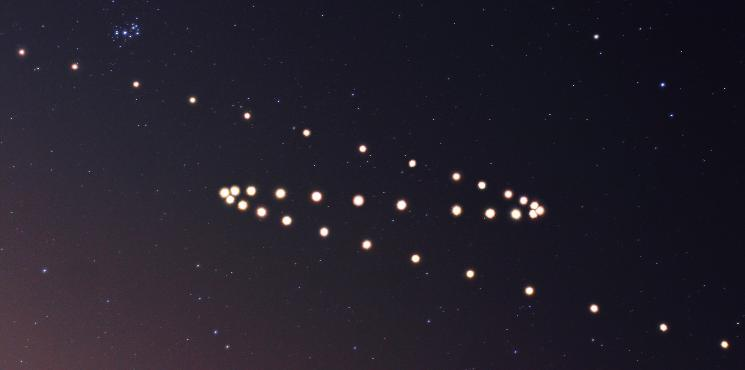
\includegraphics[width=.8\textwidth]{fig/mars_orbit.jpeg} 
\end{figure}
我们可以通过两个圆周运动的叠加来模拟出这个曲线(\url{http://faculty.fullerton.edu/cmcconnell/Planets.html}[图片来源]):
\begin{figure}[H]
  \centering
  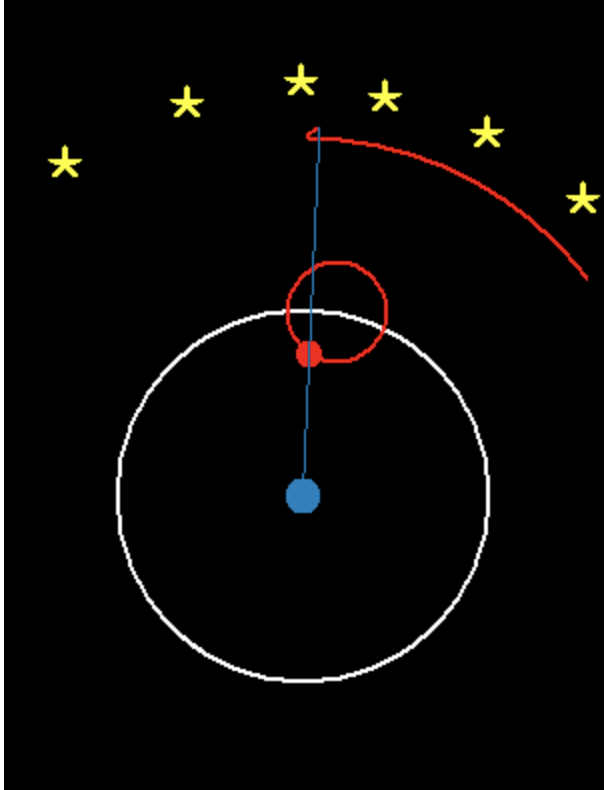
\includegraphics[width=.8\textwidth]{fig/mars_orbit_explanation.png} 
\end{figure}

其实这就是地心说。通过这种圆环套圆环的做法,可以模拟各种复杂的图形。

\subsubsection{旋转的傅立叶}
所以,傅立叶级数实际上就是把$f(x)$看作是圆周运动的组合。

只是$x$是不断变大的,而不是绕着圆变换的,所以就画出了函数曲线:
\begin{figure}[H]
  \centering
  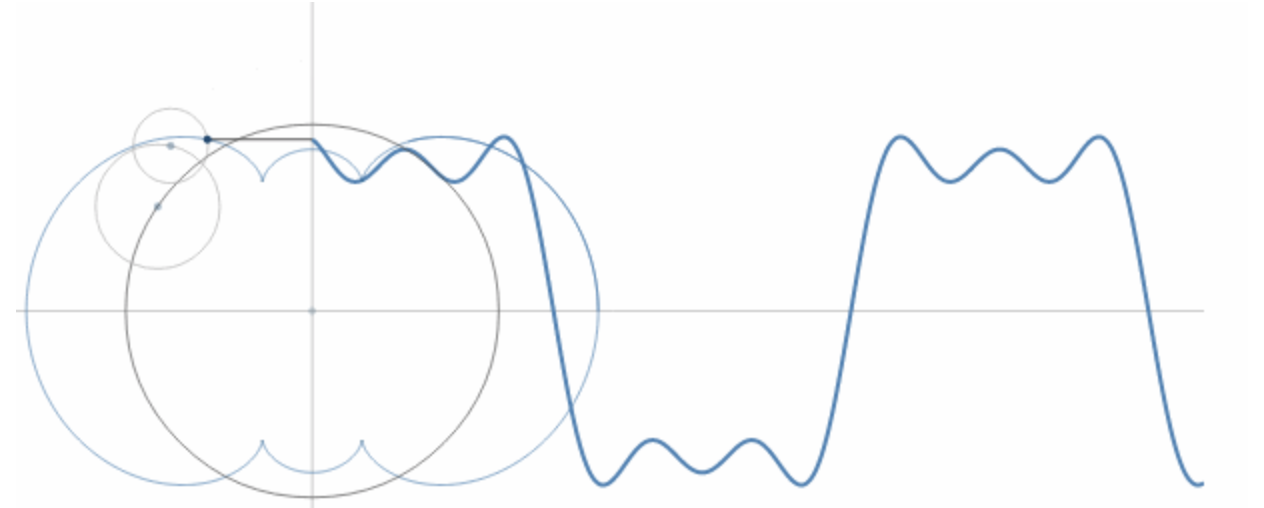
\includegraphics[width=.8\textwidth]{fig/ft_curve.png} 
\end{figure}

不断增大的$x$就好像是时间流逝,永不回头,所以我们也称为“时域”。

\subsection{频域:线性代数与傅立叶级数}
时域是现实存在的,频域却是生造的了,理解起来更加抽象。

但频域是傅立叶级数(变换)更本质的内容。

把傅立叶级数(变换)视作圆周运动的组合,是比较粗浅的看法,是买椟还珠的作法。

而把傅立叶级数(变换)看作频域,等于直接把它绑上了线性代数的战车,把它从固定在发射井中的常规核武器变成了游走不定更具威力的核潜艇、核卫星。

\subsubsection{线性代数}
线代的最基本的研究对象就是向量,带箭头的一根直线。线代的基本操作就是把向量分解为基的合成。即:
$$
\vec{u_{}}=a\vec{i_{}}+b\vec{j_{}}
$$

这么做的好处很多,比如物理中,分析各个方向上的受力,然后进行合成;比如,如果 $a >> b$,我们就可以知道,$\vec{i_{}}$上的分量更重要,$\vec{j_{}}$方向上的分量可以丢掉。(关于这个内容可以参看(“如何通俗地理解奇异值?\url{https://www.matongxue.com/madocs/306.html}”))。

\subsubsection{傅立叶级数的基}
傅立叶级数(变换)本身是线性的(这个就是比较抽象的线性了),因此我们可以把线性代数在傅立叶级数上进行推广。

让我们先找到傅立叶级数的基是什么。

为了说明方便,假设$f(x)$的周期$T=2\pi$,那么有:
$$
f(x)=\sum _{n=-\infty}^{\infty}c_{n}\cdot e^{inx}
$$

其中,以下无穷集合:
$$
\{e^{inx}\},n\in\mathbb{N}
$$

是无限维向量空间中的一组基,而且还是正交单位基。

\subsubsection{傅立叶级数向量}
$f(x)$可以写作:
$$
f(x)=\cdots+c_{-1}e^{(-1)\cdot ix}+c_{0}e^{(0)\cdot ix}+c_{1}e^{(1)\cdot ix}+c_{2}e^{(2)\cdot ix}+\cdots
$$

因为$\{e^{inx}\},n\in\mathbb{N}$是基,所以可把$f(x)$表示为一个向量:
$$
f(x)=(\cdots, c_{-1}, c_0, c_1, c_2, \cdots)
$$

这个向量其实就是傅立叶级数的向量。

因为基$\{e^{inx}\},n\in\mathbb{N}$实际上反映了周期运动的频率,我们以频率为基,所以这样看待傅立叶级数的方式就是“频域”。

\subsubsection{频谱图}
对于:
$$
f(x)=\sum _{n=-\infty}^{\infty}c_{n}\cdot e^{inx}
$$

我们用$(n,c_n)$来描点作图,就得到频谱图。

下面是一个周期矩形波的频谱图(右图中的实线部分是频谱图,虚线是拟合的频谱的趋势):
\begin{figure}[H]
  \centering
  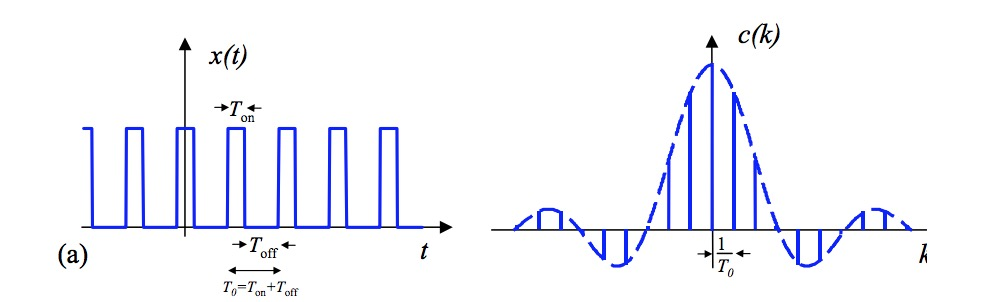
\includegraphics[width=.8\textwidth]{fig/square_wave.png}
\end{figure}

\subsection{傅立叶级数和傅立叶变换}
傅立叶级数是基于周期函数的,如果我们把周期推广到$\infty$,那么也就变为了非周期函数,这就是傅立叶变换。

两者的频谱图对比,可以看到傅立叶变换的频谱图是连续的(上面是周期函数的傅立叶级数分解[右边的实线是频谱,虚线是拟合的频谱的趋势],下面是非周期函数的傅立叶变换[只有实线的频谱]):
\begin{figure}[H]
  \centering
  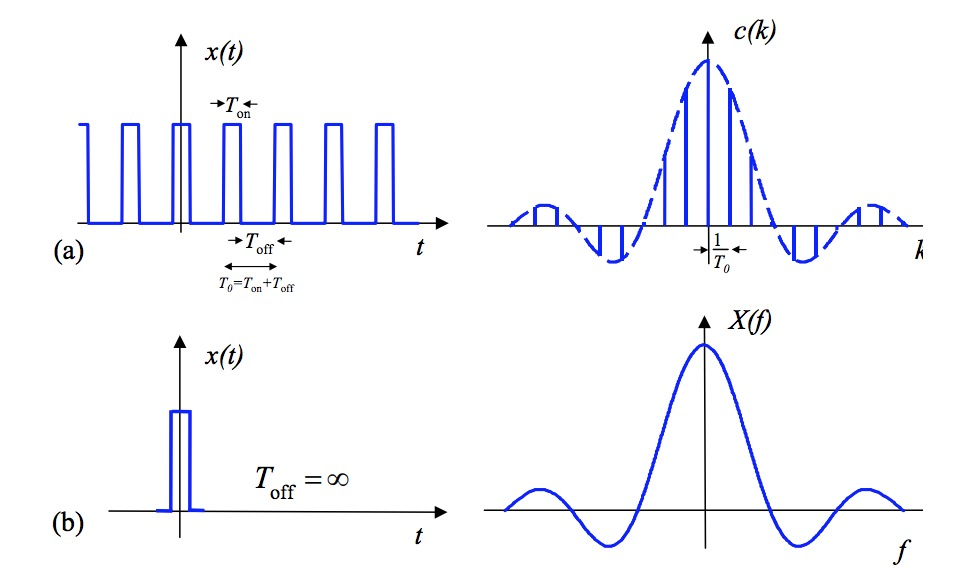
\includegraphics[width=.8\textwidth]{fig/ft_continuous_compare.png} 
\end{figure}




\url{https://www.matongxue.com/madocs/712.html}

\url{https://www.matongxue.com/madocs/723.html}

%\printbibliography
\bibliography{../ref}
\bibliographystyle{IEEEtran}
\end{document}
